\documentclass{beamer}

\mode<presentation>
{
  \usetheme{Berlin}
  \usecolortheme{orchid}
  \setbeamercovered{transparent}
}

\usepackage[english]{babel}
\usepackage[latin1]{inputenc}
\usepackage{times}
\usepackage{fontenc} 
% Or whatever. Note that the encoding and the font should match. If T1
% does not look nice, try deleting the line with the fontenc.
\usepackage{amsmath}

\newcommand{\linespace}{\vskip 0.25cm}

\definecolor{MyForestGreen}{rgb}{0,0.7,0} 
\newcommand{\tableemph}[1]{{#1}}
\newcommand{\tablewin}[1]{\tableemph{#1}}
\newcommand{\tablemid}[1]{\tableemph{#1}}
\newcommand{\tablelose}[1]{\tableemph{#1}}

\definecolor{MyLightGray}{rgb}{0.6,0.6,0.6}
\newcommand{\tabletie}[1]{\color{MyLightGray} {#1}}

% The text in square brackets is the short version of your title and will be used in the
% header/footer depending on your theme.
\title{Applying Genetic Programming to\\ Bytecode and Assembly}

% Sub-titles are optional - uncomment and edit the next line if you want one.
% \subtitle{Why does sub-tree crossover work?} 

% The text in square brackets is the short version of your name(s) and will be used in the
% header/footer depending on your theme.
\author{Eric Collom}

% The text in square brackets is the short version of your institution and will be used in the
% header/footer depending on your theme.
\institute[University of Minnesota, Morris]
{
  Division of Science and Mathematics \\
  University of Minnesota, Morris \\
  Morris, Minnesota, USA
}

% The text in square brackets is the short version of the date if you need that.
\date{29 April '14,\\ UMM Senior Seminar}

% Delete this, if you do not want the table of contents to pop up at
% the beginning of each subsection:
\AtBeginSection[]
{
  \begin{frame}<beamer>
    \frametitle{Outline}
    \tableofcontents[currentsection, hideothersubsections]
  \end{frame}
}

\begin{document}

\begin{frame}
  \titlepage
\end{frame}

% For a 20-25 minute senior seminar talk you probably want something like:
% - Two or three major sections (other than the summary).
% - At *most* three subsections per section.resentation, people show regularly a "outline" frame containing the table of contents where some sections are grey (have been presented) and others are highlighted (will be presented right now).
% - Talk about 30s to 2min per frame. So there should probably be between
%   15 and 30 frames, all told.

\section*{Overview}

\subsection*{The big picture}

\begin{frame}
  \frametitle{The big picture}

  \begin{itemize}  
  	\item Evolving whole programs is hard to do with source code.
	\item Evolving whole programs with bytecode and assembly is not as hard.
  \end{itemize}

%   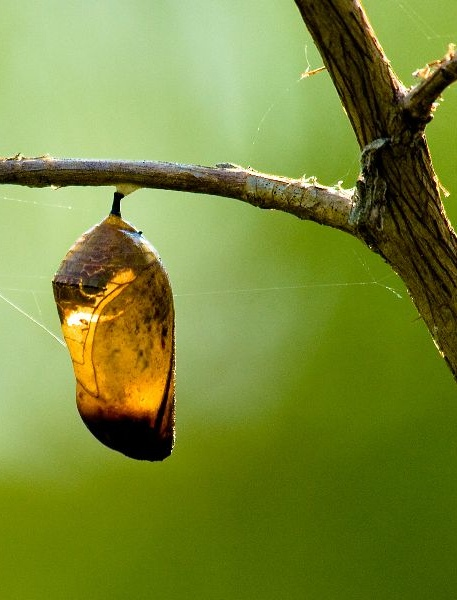
\includegraphics[width=0.95\textwidth]{Illustrations/Empty_cocoon_crop_by_Bluedrakon_from_Flickr.jpg}
%       \\
%    \only{\tiny{Bluedrakon \\ \url{http://tr.im/pWUi} }}

\end{frame}

\subsection*{Outline}

\begin{frame}
  \frametitle{Outline}
  \tableofcontents[hideallsubsections]
\end{frame}

\section[Background]{Background}

\subsection[EC]{EC}

\begin{frame}
  \frametitle{What is Evolutionary Computation?}
  \begin{columns}
  \begin{column}{0.6\textwidth}
  \begin{itemize}
  	\item EC is a a technique that is used to automate computer problem solving.
  	\item Loosely emulates evolutionary biology.
  \end{itemize}
  \end{column}
  \begin{column}{0.4\textwidth}
   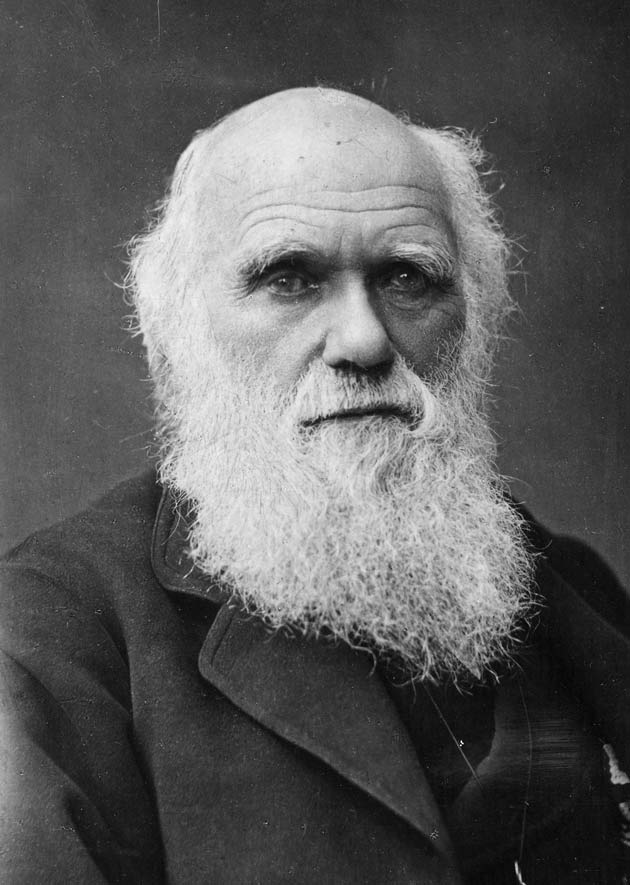
\includegraphics[width=0.95\textwidth]{Illustrations/darwin.jpg}
       \\
    \only{\tiny{Charles Darwin \\ \url{http://tinyurl.com/lqwj3wt} }}
  \end{column}
  \end{columns}
\end{frame}

\begin{frame}
	\frametitle{How does it work}
\begin{columns}
\begin{column}{0.6\textwidth}
\begin{itemize}	
	\item Continuous Optimization
	\item Selection is driven by the \textit{fitness} of individuals
	\item Genetic Operators mimic sexual reproduction and mutation
	
\end{itemize}
\end{column}
\begin{column}{0.4\textwidth}
   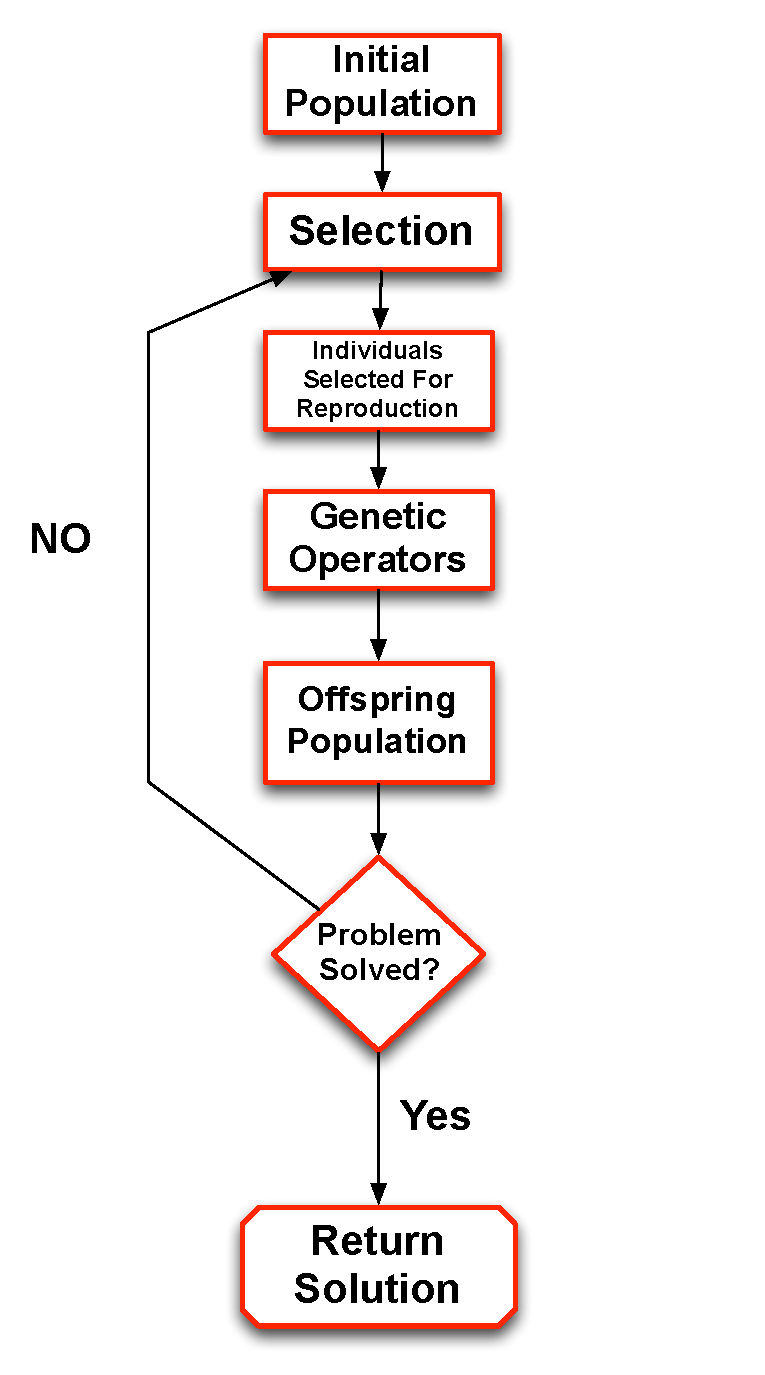
\includegraphics[height=0.90\textheight]{Illustrations/ECdiagram.pdf}
       \\
   \only{\tiny{The Evolutionary Computation Process}}
\end{column}
\end{columns}

\end{frame}

\begin{frame}
	\frametitle{Genetic Programming}
\begin{columns}
\begin{column}{0.5\textwidth}
\begin{itemize}	
	\item Uses the EC technique to evolve programs
	\item The population is programs
	
\end{itemize}
\end{column}
\begin{column}{0.5\textwidth}
   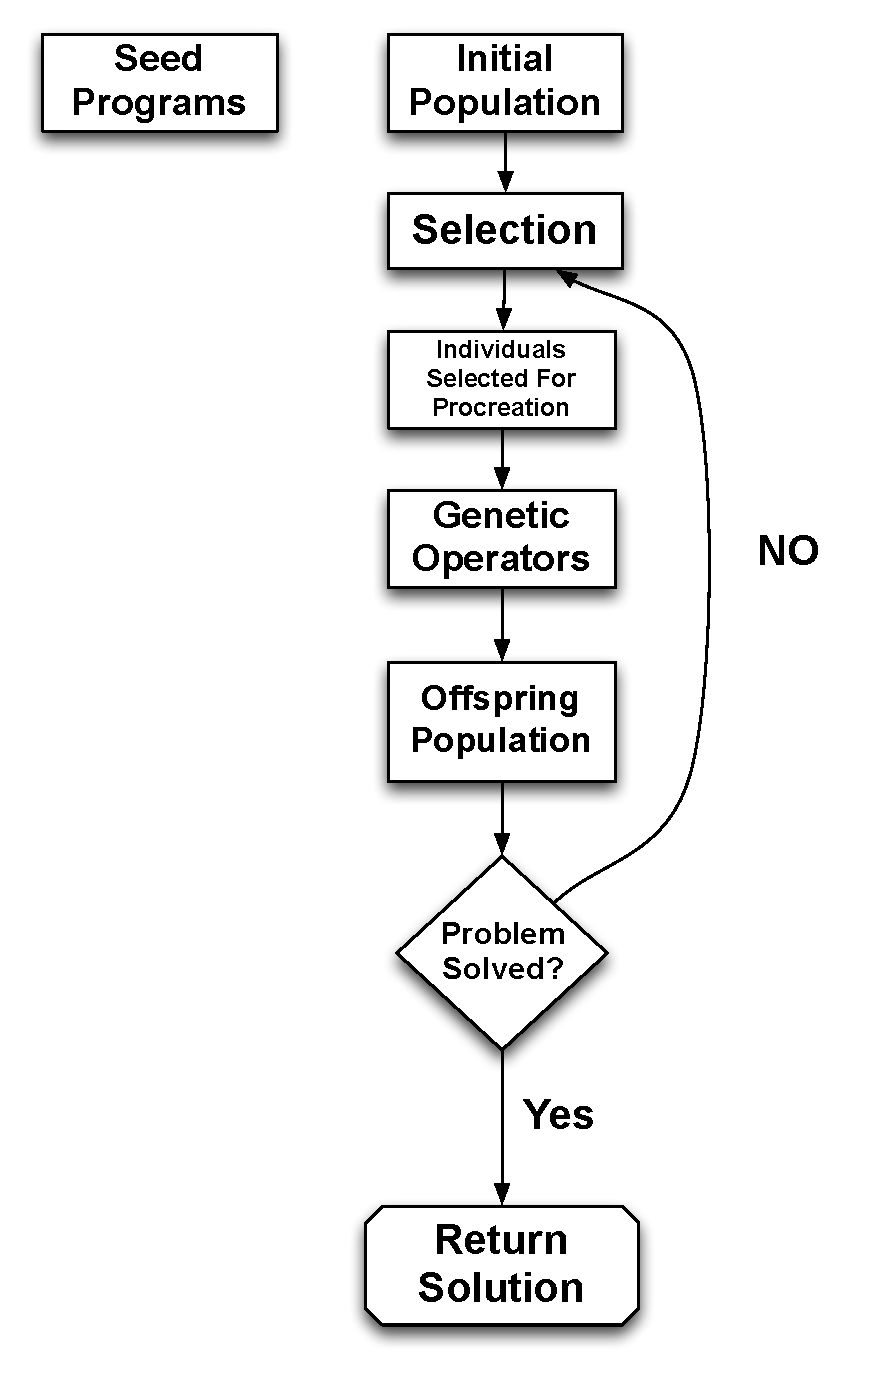
\includegraphics[height=0.90\textheight]{Illustrations/GP1.pdf}
       \\
   \only{\tiny{The Evolutionary Computation Process}}
\end{column}
\end{columns}

\end{frame}

\begin{frame}
	\frametitle{Genetic Programming}
\begin{columns}
\begin{column}{0.5\textwidth}
\begin{itemize}	
	\item Tournament Selection
	
\end{itemize}
\end{column}
\begin{column}{0.5\textwidth}
   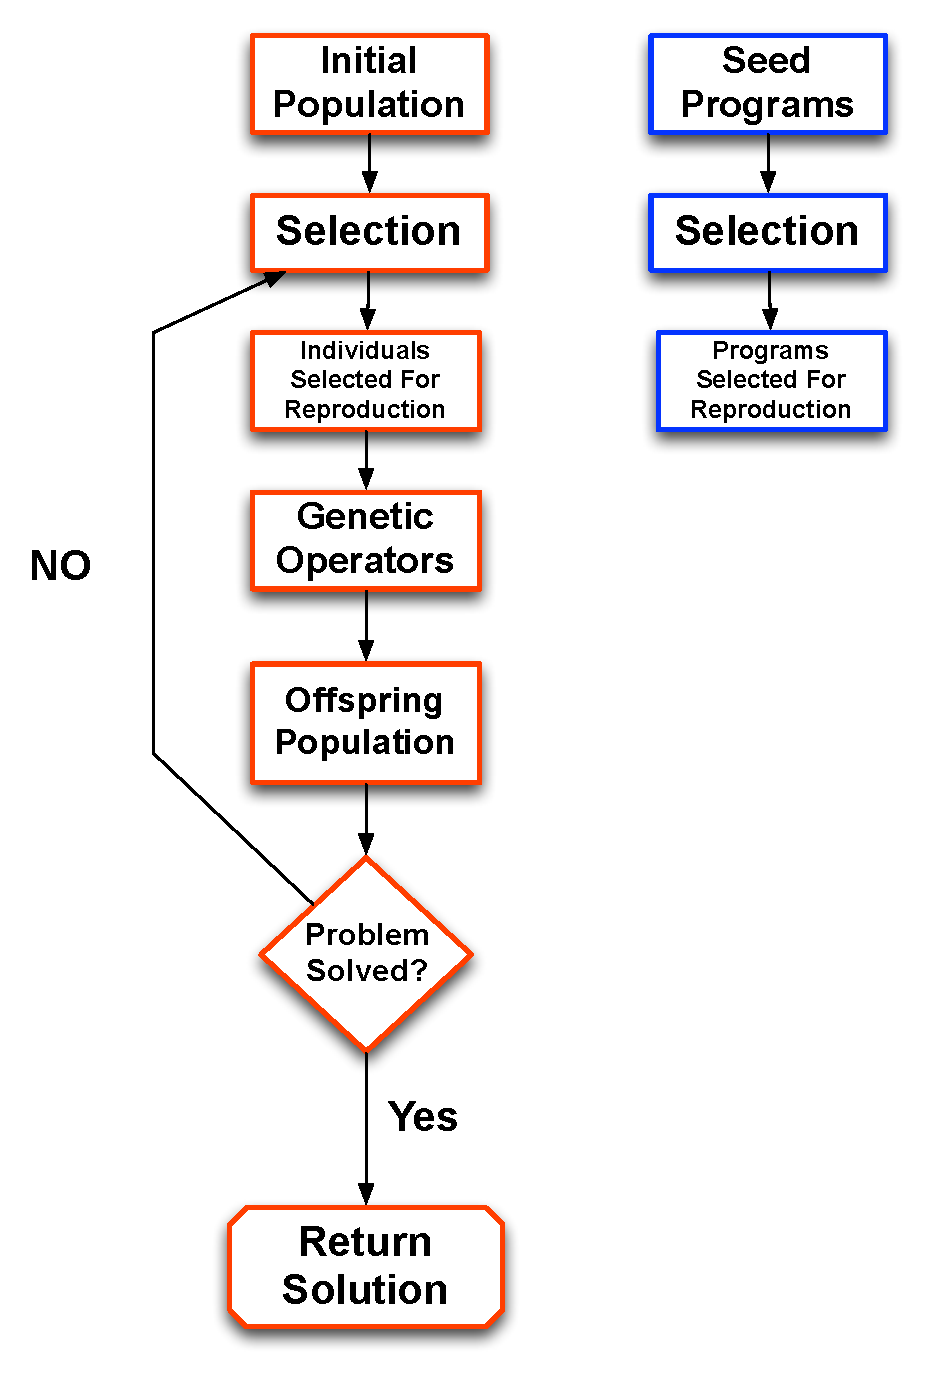
\includegraphics[height=0.90\textheight]{Illustrations/GP2.pdf}
       \\
   \only{\tiny{The Evolutionary Computation Process}}
\end{column}
\end{columns}

\end{frame}

\begin{frame}
	\frametitle{Genetic Programming}
\begin{columns}
\begin{column}{0.5\textwidth}
\begin{itemize}	
	\item Crossover
	\item Mutation
\end{itemize}
\end{column}
\begin{column}{0.5\textwidth}
   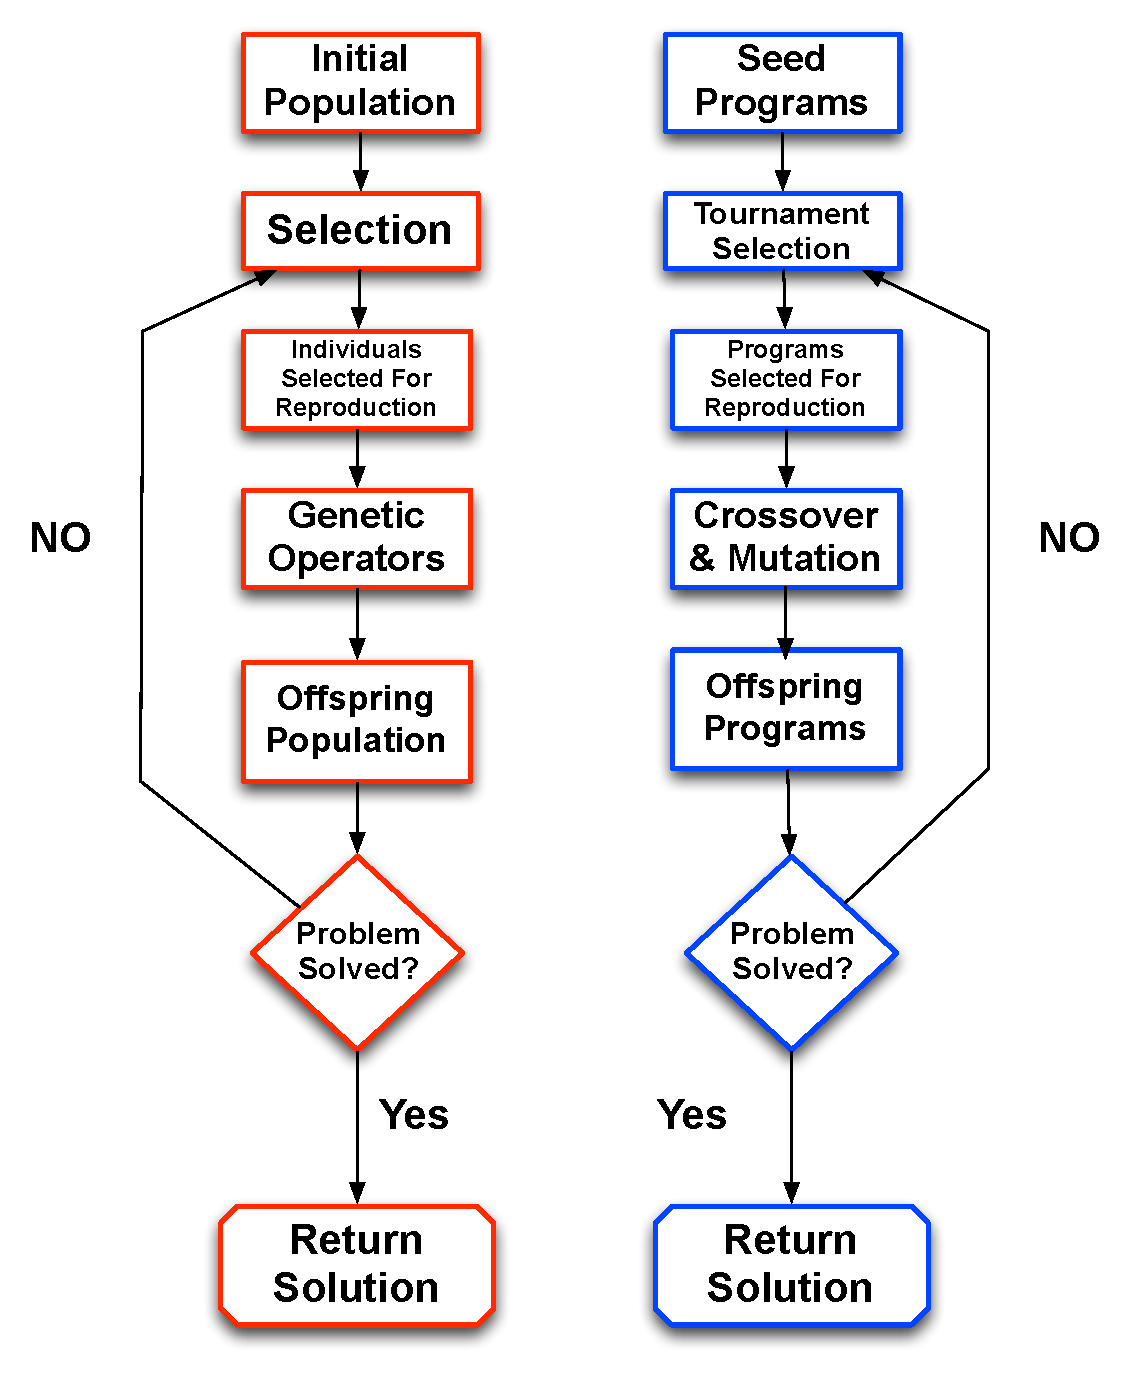
\includegraphics[height=0.90\textheight]{Illustrations/GP3.pdf}
       \\
   \only{\tiny{The Evolutionary Computation Process}}
\end{column}
\end{columns}

\end{frame}

\begin{frame}
	\frametitle{Crossover}

   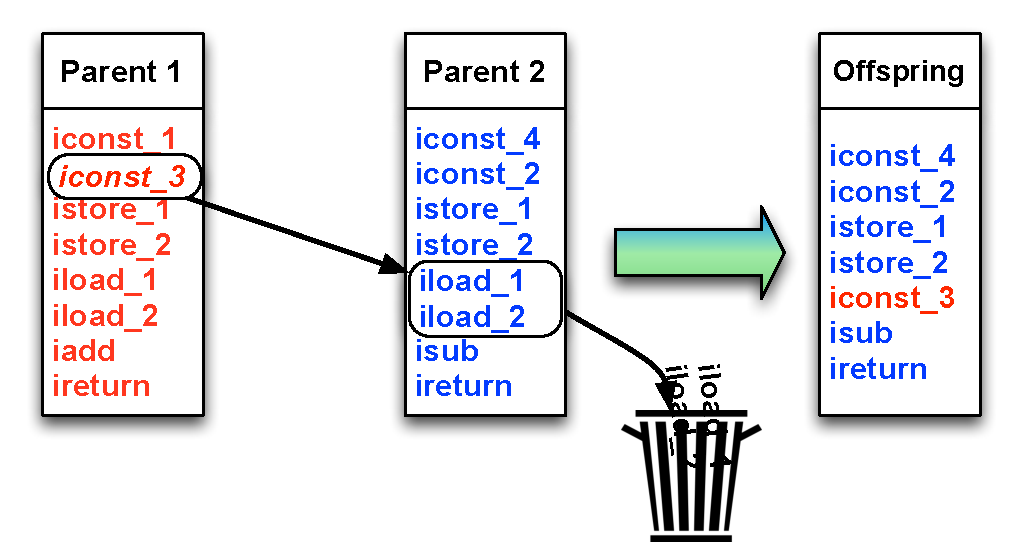
\includegraphics[width=1\textwidth]{Illustrations/crossover.pdf}
       \\
   \only{\tiny{Crossover with Java Bytecode}}

\end{frame}

\begin{frame}
	\frametitle{Mutation}

   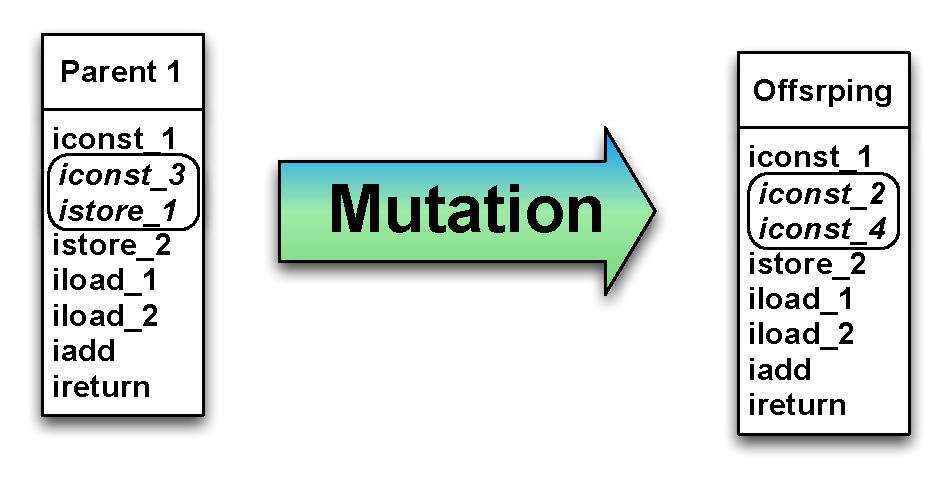
\includegraphics[width=1\textwidth]{Illustrations/mutation.pdf}
       \\
   \only{\tiny{Crossover with Java Bytecode}}

\end{frame}






\subsection[Bytecode and Assembly]{Java Bytecode and x86 Assembly}

\begin{frame}
	\frametitle{Java Virtual Machine}

\begin{itemize}	
\item Frames
\item Array of local variables
\item Operand Stack

\end{itemize}

\end{frame}



\begin{frame}
\frametitle{Java Bytcode and Frames}
\begin{columns}
\begin{column}{0.5\textwidth}
\begin{itemize}	
\item Opcodes
\item Prefix indicates type
\end{itemize}
\end{column}

\begin{column}{0.5\textwidth}
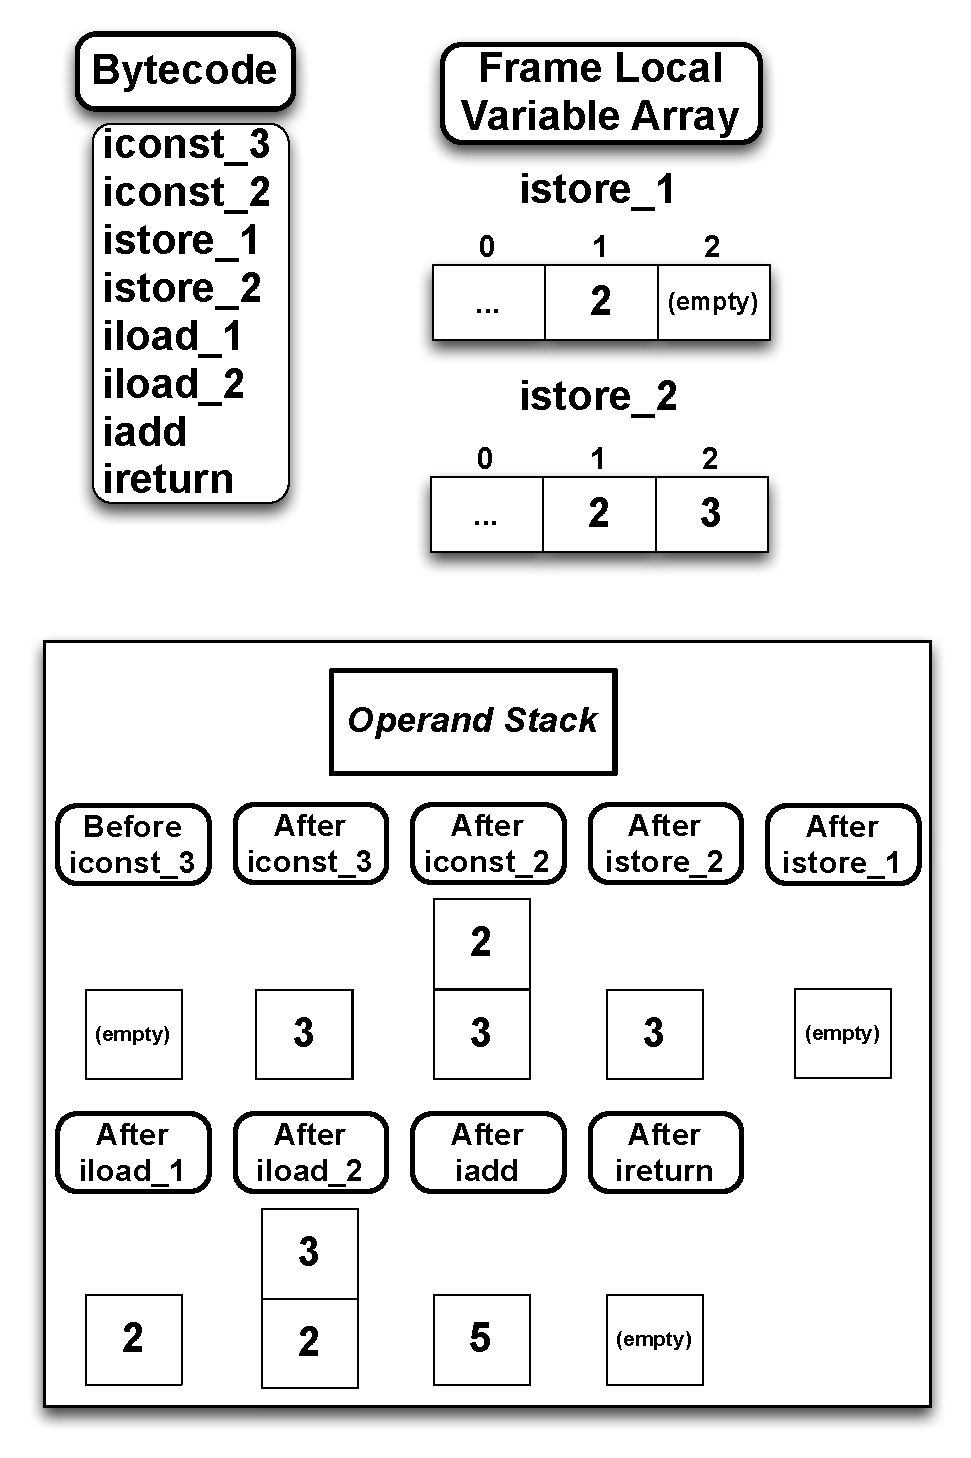
\includegraphics[height=.8\textheight]{Illustrations/stackBytecode.pdf}
\end{column}
\end{columns}
\end{frame}

\section[Why Instruction-level code]{Why Evolve Instruction-level Code}

\begin{frame}
	\frametitle{Source Code Constraints}
\end{frame}

\begin{frame}
	\frametitle{Flexibility}
\end{frame}

\section[FINCH]{FINCH:Evolving Programs}

\subsection[How it works]{How it Works}
\begin{frame}
  \frametitle{Selecting Offspring}
  
  \begin{columns}
  \begin{column}{0.6\textwidth}
  \begin{itemize}
  	\item There is still a chance to produce non-compilable code
	\item Solution: Add restrictions to code selection.
	\item Stack and Frame Depth
	\item Variable Types
	\item Control Flow
  \end{itemize}
  \end{column}
  \begin{column}{0.4\textwidth}
	  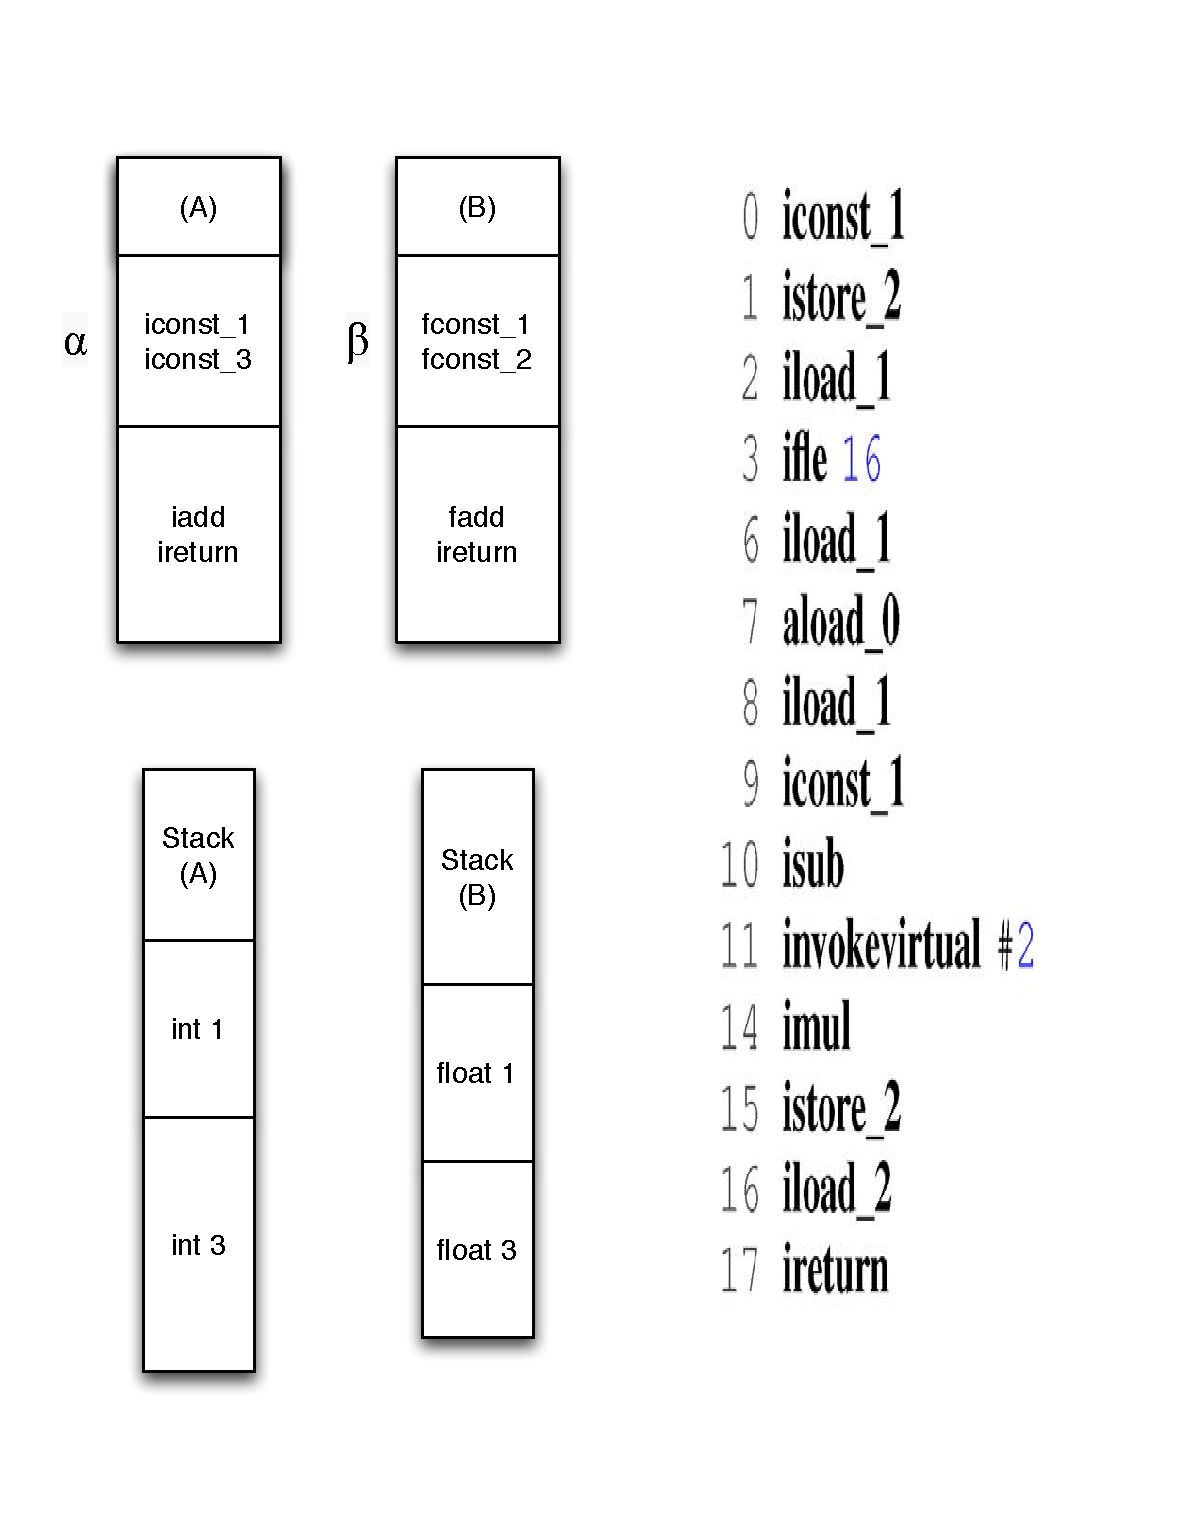
\includegraphics[width=0.95\textwidth]{talk.pdf}
  \end{column}
	  
  
  \end{columns}
\end{frame}

\begin{frame}
  \frametitle{Crossover}
\end{frame}

\begin{frame}
\frametitle{Non-Halting Offspring}
\end{frame}

\subsection[Results]{Results}


\section[Evolving Assembly]{Using Instruction-level code to automate bug repair}

\subsection{How it Works}
\begin{frame}
  \frametitle{Selecting Offspring}
\end{frame}

\begin{frame}
  \frametitle{Genetic Operators}
\end{frame}

\begin{frame}
  \frametitle{Non-Halting Offspring}
\end{frame}

\subsection[Results]{Results}

\section[Conclusions]{Conclusions}

\begin{frame}
\frametitle{Conclusions}
\end{frame}

\section*{References}

\begin{frame} 
	\frametitle{References} 
	
	\begin{thebibliography}{lskdjf}
  	\end{thebibliography}
\end{frame} 

\end{document}


